\documentclass[tikz,border=8pt]{standalone}
% Shared look for every TikZ diagram. Load with \input{../../tools/tikz-style.tex}
\usepackage[sfdefault]{roboto}
\usetikzlibrary{arrows.meta, positioning, shapes.geometric, calc, fit, backgrounds}
\definecolor{cblue}{HTML}{4C78A8}
\definecolor{corange}{HTML}{F58518}
\definecolor{cgreen}{HTML}{54A24B}
\definecolor{cred}{HTML}{E45756}
\definecolor{cpurple}{HTML}{B279A2}
\definecolor{cgrey}{HTML}{6B6B6B}
\tikzset{
  every picture/.style={font=\sffamily, line width=1.2pt},
  box/.style={draw=#1, fill=#1!12, rounded corners=4pt, align=center, inner sep=7pt, minimum height=1.1cm},
  box/.default=cgrey,
  arrow/.style={-{Stealth[length=3mm]}, draw=cgrey, line width=1.4pt},
  title/.style={font=\sffamily\bfseries\Large},
  note/.style={font=\sffamily\small, text=cgrey, align=center},
}
\AtBeginDocument{\hyphenpenalty=10000 \exhyphenpenalty=10000}

% Figure 5: the speed loop's block diagram (laid out as block_diagram.tex) with the seven stages of one 10 ms cycle
% numbered in the order the computer runs them, and each signal's value in the first cycle on the ramp, t = 4.00 s
% (closed-loop ramp run of speedkit.py, no sensor noise; the notebook prints every value).
% loop_cycles.py reuses this file for Figure 6: it redefines the values below, turns the stages off and adds its plots
% at the FRAME line.
\newcommand{\vTitle}{the first cycle on the ramp, $t = 4.00$ s}
\newcommand{\vM}{0.500 m/s}
\newcommand{\vE}{0 m/s}
\newcommand{\vU}{1 N}
\newcommand{\vF}{1 N}
\newcommand{\vPlant}{drag 1 N\\ net force $-0.785$ N}
\newcommand{\vY}{new speed\\ 0.49902 m/s}
\newif\ifstages \stagestrue
\begin{document}
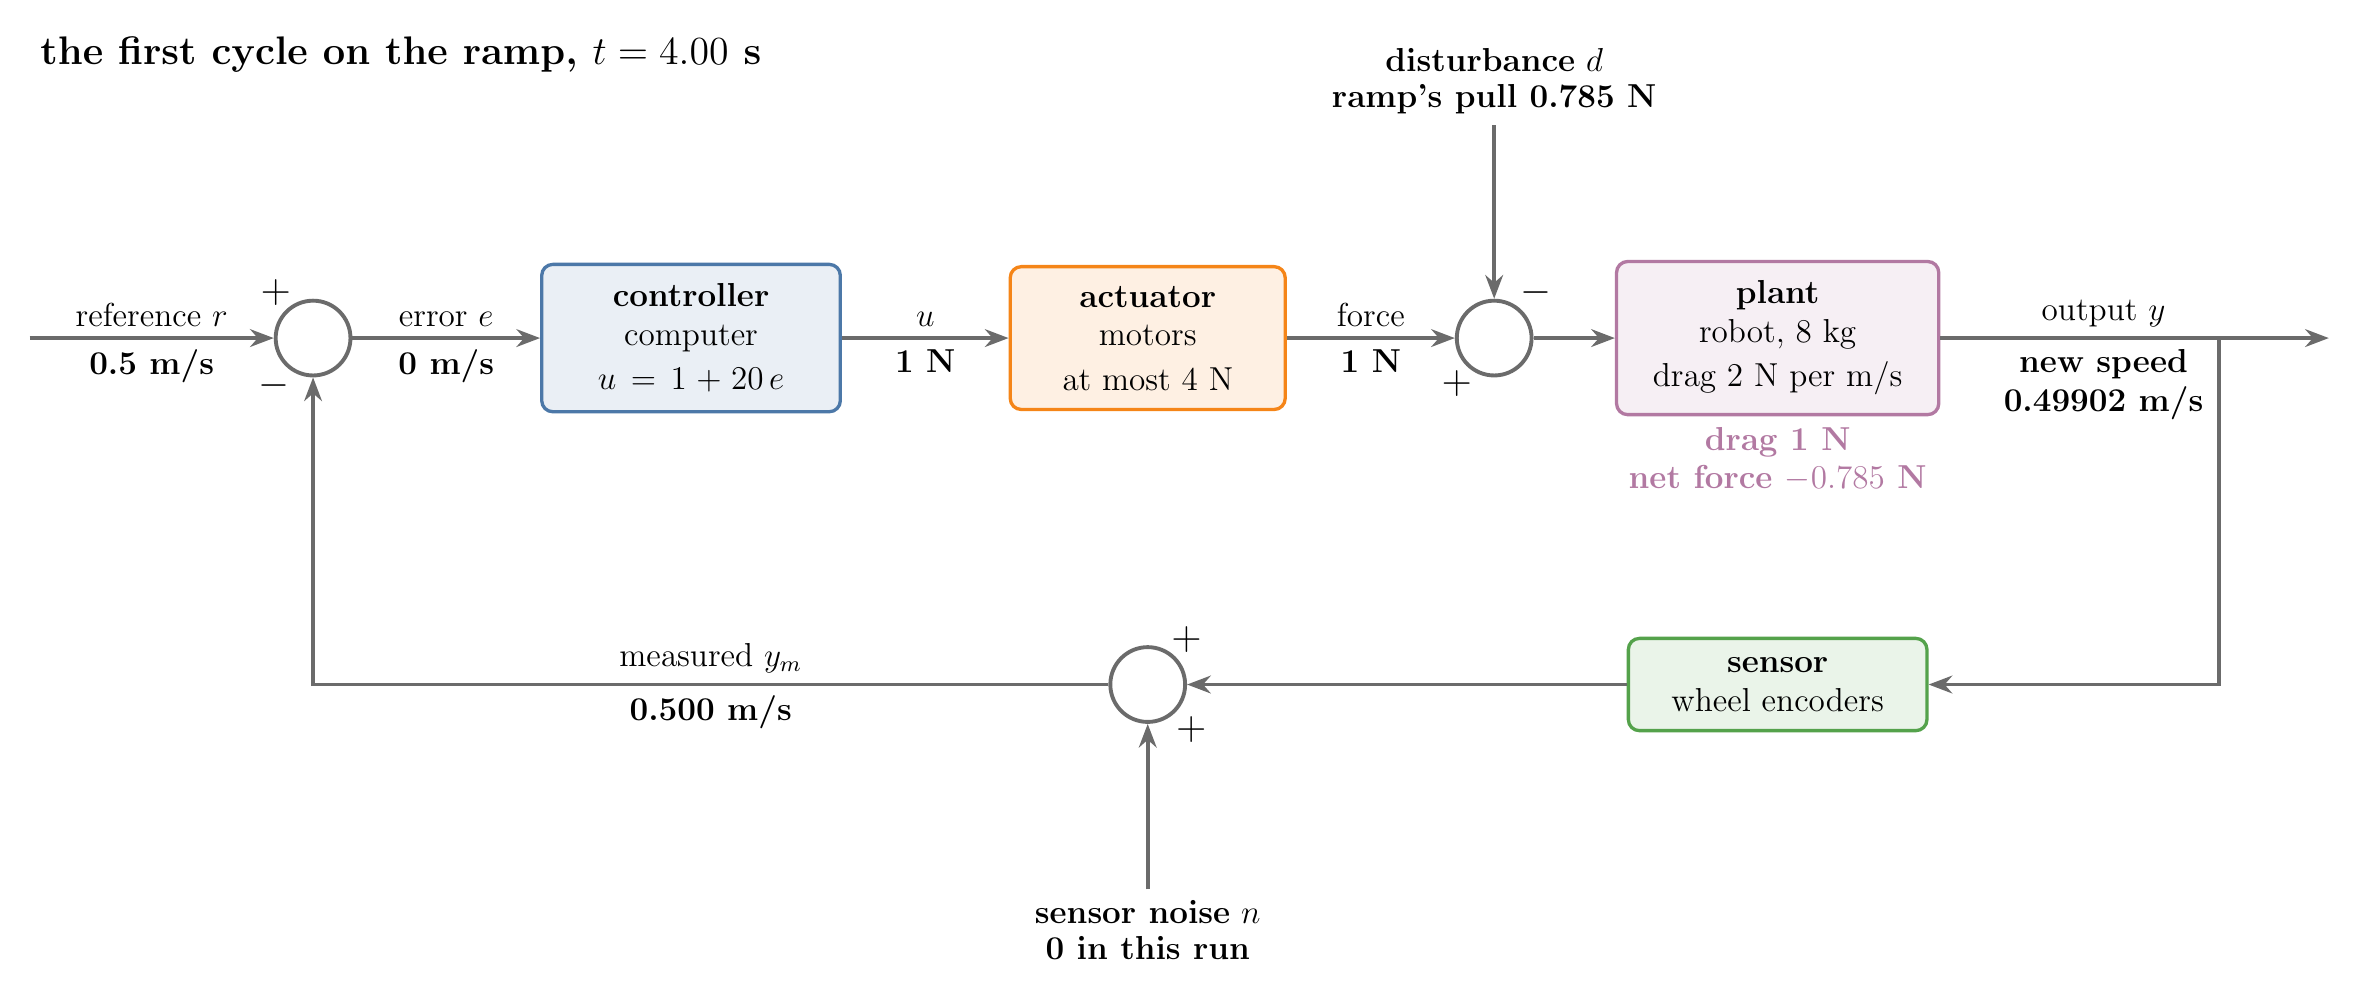
\begin{tikzpicture}[every node/.append style={font=\large},
    sum/.style={circle, draw=cgrey, fill=white, minimum size=0.95cm, inner sep=0pt, line width=1.4pt},
    val/.style={font=\large\bfseries, align=center},
    stage/.style={circle, fill=black, text=white, font=\normalsize\bfseries, inner sep=0pt, minimum size=0.66cm}]
  \node[font=\Large\bfseries, anchor=west] at (-1.0,3.6) {\vTitle};
  % top row: forward path
  \node[sum] (s1) at (2.6,0) {};
  \node[box=cblue, text width=3.3cm] (ctrl) at (7.4,0) {\textbf{controller}\\ computer\\[2pt] $u = 1 + 20\,e$};
  \node[box=corange, text width=3.0cm] (act) at (13.2,0) {\textbf{actuator}\\ motors\\[2pt] at most 4 N};
  \node[sum] (s2) at (17.6,0) {};
  \node[box=cpurple, text width=3.6cm] (plant) at (21.2,0) {\textbf{plant}\\ robot, 8 kg\\[2pt] drag 2 N per m/s};
  \node[val, text=cpurple, anchor=north] at (plant.south) {\vPlant};
  % bottom row: feedback path
  \node[box=cgreen, text width=3.3cm] (sens) at (21.2,-4.4) {\textbf{sensor}\\ wheel encoders};
  \node[sum] (s3) at (13.2,-4.4) {};
  % signals, each with its value below the arrow
  \draw[arrow] (-1.0,0) -- node[above] {reference $r$} node[below, val] {0.5 m/s} (s1.west);
  \node[font=\Large] at ($(s1.north west)+(-0.12,0.22)$) {$+$};
  \node[font=\Large] at ($(s1.south west)+(-0.14,-0.25)$) {$-$};
  \draw[arrow] (s1.east) -- node[above] {error $e$} node[below, val] {\vE} (ctrl.west);
  \draw[arrow] (ctrl.east) -- node[above] {$u$} node[below, val] {\vU} (act.west);
  \draw[arrow] (act.east) -- node[above] {force} node[below, val] {\vF} (s2.west);
  \node[font=\Large] at ($(s2.south west)+(-0.12,-0.22)$) {$+$};
  \node[font=\Large] at ($(s2.north east)+(0.18,0.22)$) {$-$};
  \draw[arrow] (17.6,2.7) node[above, align=center] {\textbf{disturbance} $d$\\[-1pt] \textbf{ramp's pull 0.785 N}}
     -- (s2.north);
  \draw[arrow] (s2.east) -- (plant.west);
  \draw[arrow] (plant.east) -- node[pos=0.42, above] {output $y$} node[pos=0.42, below, val] {\vY} (28.2,0);
  \draw[arrow] (26.8,0) -- (26.8,-4.4) -- (sens.east);
  \draw[arrow] (sens.west) -- (s3.east);
  \node[font=\Large] at ($(s3.north east)+(0.14,0.22)$) {$+$};
  \node[font=\Large] at ($(s3.south east)+(0.2,-0.22)$) {$+$};
  \draw[arrow] (13.2,-7.0) node[below, align=center] {\textbf{sensor noise} $n$\\[-1pt] \textbf{0 in this run}}
     -- (s3.south);
  \draw[arrow] (s3.west) -- node[above] {measured $y_m$} node[below, val] {\vM} (2.6,-4.4) -- (s1.south);
  \ifstages
  % the seven stages of one cycle, in the order the computer runs them
  \node[stage] at (0.55,1.2) {1};
  \node[stage] at (sens.north west) {2};
  \node[stage] at (2.6,1.15) {3};
  \node[stage] at (ctrl.north west) {4};
  \node[stage] at (act.north west) {5};
  \node[stage] at (plant.north west) {6};
  \node[stage] at (27.45,-2.2) {7};
  \foreach \i/\x/\y/\t in {1/-0.6/-9.2/the plan gives the reference $r$,
                          2/-0.6/-10.1/the encoders measure the speed,
                          3/-0.6/-11.0/the summing junction forms the error $e$,
                          4/-0.6/-11.9/the computer computes the push $u$,
                          5/14.0/-9.2/the motors push,
                          6/14.0/-10.1/{push, ramp's pull and drag change the speed for 10 ms},
                          7/14.0/-11.0/the new speed goes to the sensor for the next cycle} {
    \node[stage] at (\x,\y) {\i};
    \node[anchor=west, font=\Large] at (\x+0.45,\y) {\t};
  }
  \fi
  % FRAME
\end{tikzpicture}
\end{document}
